\chapter{Caminos y circuitos}

Este capítulo se centra en dos tipos de caminos en grafos:
\begin{itemize}
\item Un camino \key{Euleriano} es un camino que
atraviesa cada arista exactamente una vez.
\item Un camino \key{Hamiltoniano} es un camino
que visita cada nodo exactamente una vez.
\end{itemize}

Si bien los caminos Eulerianos y Hamiltonianos parecen
conceptos similares a primera vista,
los problemas computacionales relacionados con ellos
son muy diferentes.
Resulta que hay una regla simple que
determina si un grafo contiene un camino Euleriano,
y también existe un algoritmo eficiente para
encontrar dicho camino si existe.
Por el contrario, verificar la existencia de un camino Hamiltoniano es un problema NP-difícil,
y no se conoce ningún algoritmo eficiente para resolver el problema.

\section{Caminos Eulerianos}

\index{Camino Euleriano}

Un camino \key{Euleriano}\footnote{L. Euler estudió este tipo de caminos en 1736
cuando resolvió el famoso problema de los puentes de Königsberg.
Este fue el nacimiento de la teoría de grafos.} es un camino
que atraviesa exactamente una vez cada arista del grafo.
Por ejemplo, el grafo
\begin{center}
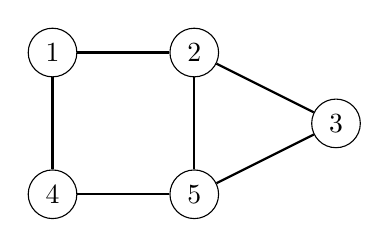
\begin{tikzpicture}[scale=0.9]
\node[draw, circle] (1) at (1,5) {$1$};
\node[draw, circle] (2) at (3,5) {$2$};
\node[draw, circle] (3) at (5,4) {$3$};
\node[draw, circle] (4) at (1,3) {$4$};
\node[draw, circle] (5) at (3,3) {$5$};

\path[draw,thick,-] (1) -- (2);
\path[draw,thick,-] (2) -- (3);
\path[draw,thick,-] (1) -- (4);
\path[draw,thick,-] (3) -- (5);
\path[draw,thick,-] (2) -- (5);
\path[draw,thick,-] (4) -- (5);
\end{tikzpicture}
\end{center}
tiene un camino Euleriano desde el nodo 2 hasta el nodo 5:
\begin{center}
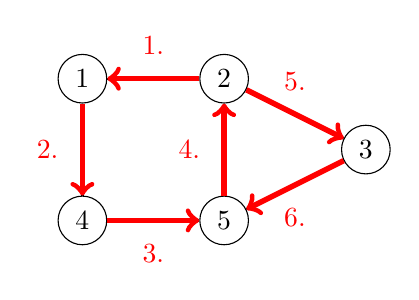
\begin{tikzpicture}[scale=0.9]
\node[draw, circle] (1) at (1,5) {$1$};
\node[draw, circle] (2) at (3,5) {$2$};
\node[draw, circle] (3) at (5,4) {$3$};
\node[draw, circle] (4) at (1,3) {$4$};
\node[draw, circle] (5) at (3,3) {$5$};

\path[draw,thick,-] (1) -- (2);
\path[draw,thick,-] (2) -- (3);
\path[draw,thick,-] (1) -- (4);
\path[draw,thick,-] (3) -- (5);
\path[draw,thick,-] (2) -- (5);
\path[draw,thick,-] (4) -- (5);

\path[draw=red,thick,->,line width=2pt] (2) -- node[font=\small,label={[red]north:1.}] {} (1);
\path[draw=red,thick,->,line width=2pt] (1) -- node[font=\small,label={[red]left:2.}] {} (4);
\path[draw=red,thick,->,line width=2pt] (4) -- node[font=\small,label={[red]south:3.}] {} (5);
\path[draw=red,thick,->,line width=2pt] (5) -- node[font=\small,label={[red]left:4.}] {} (2);
\path[draw=red,thick,->,line width=2pt] (2) -- node[font=\small,label={[red]north:5.}] {} (3);
\path[draw=red,thick,->,line width=2pt] (3) -- node[font=\small,label={[red]south:6.}] {} (5);
\end{tikzpicture}
\end{center}
\index{Circuito Euleriano}
Un \key{circuito Euleriano}
es un camino Euleriano que comienza y termina
en el mismo nodo.
Por ejemplo, el grafo
\begin{center}
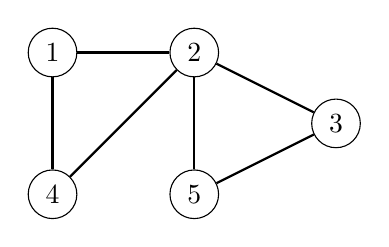
\begin{tikzpicture}[scale=0.9]
\node[draw, circle] (1) at (1,5) {$1$};
\node[draw, circle] (2) at (3,5) {$2$};
\node[draw, circle] (3) at (5,4) {$3$};
\node[draw, circle] (4) at (1,3) {$4$};
\node[draw, circle] (5) at (3,3) {$5$};

\path[draw,thick,-] (1) -- (2);
\path[draw,thick,-] (2) -- (3);
\path[draw,thick,-] (1) -- (4);
\path[draw,thick,-] (3) -- (5);
\path[draw,thick,-] (2) -- (5);
\path[draw,thick,-] (2) -- (4);
\end{tikzpicture}
\end{center}
tiene un circuito Euleriano que comienza y termina en el nodo 1:
\begin{center}
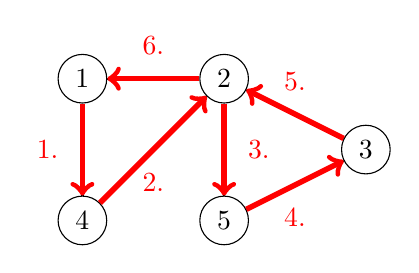
\begin{tikzpicture}[scale=0.9]
\node[draw, circle] (1) at (1,5) {$1$};
\node[draw, circle] (2) at (3,5) {$2$};
\node[draw, circle] (3) at (5,4) {$3$};
\node[draw, circle] (4) at (1,3) {$4$};
\node[draw, circle] (5) at (3,3) {$5$};

\path[draw,thick,-] (1) -- (2);
\path[draw,thick,-] (2) -- (3);
\path[draw,thick,-] (1) -- (4);
\path[draw,thick,-] (3) -- (5);
\path[draw,thick,-] (2) -- (5);
\path[draw,thick,-] (2) -- (4);

\path[draw=red,thick,->,line width=2pt] (1) -- node[font=\small,label={[red]left:1.}] {} (4);
\path[draw=red,thick,->,line width=2pt] (4) -- node[font=\small,label={[red]south:2.}] {} (2);
\path[draw=red,thick,->,line width=2pt] (2) -- node[font=\small,label={[red]right:3.}] {} (5);
\path[draw=red,thick,->,line width=2pt] (5) -- node[font=\small,label={[red]south:4.}] {} (3);
\path[draw=red,thick,->,line width=2pt] (3) -- node[font=\small,label={[red]north:5.}] {} (2);
\path[draw=red,thick,->,line width=2pt] (2) -- node[font=\small,label={[red]north:6.}] {} (1);
\end{tikzpicture}
\end{center}

\subsubsection{Existencia}

La existencia de caminos y circuitos Eulerianos
depende de los grados de los nodos.
Primero, un grafo no dirigido tiene un camino Euleriano 
exactamente cuando todas las aristas
pertenecen al mismo componente conectado y
\begin{itemize}
\item el grado de cada nodo es par \emph{o}
\item el grado de exactamente dos nodos es impar,
y el grado de todos los demás nodos es par.
\end{itemize}

En el primer caso, cada camino Euleriano es también un circuito Euleriano.
En el segundo caso, los nodos de grado impar son los nodos de inicio
y finalización de un camino Euleriano que no es un circuito Euleriano.
\begin{samepage}
Por ejemplo, en el gráfico
\begin{center}
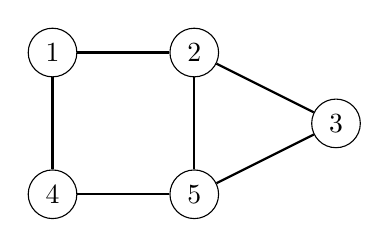
\begin{tikzpicture}[scale=0.9]
\node[draw, circle] (1) at (1,5) {$1$};
\node[draw, circle] (2) at (3,5) {$2$};
\node[draw, circle] (3) at (5,4) {$3$};
\node[draw, circle] (4) at (1,3) {$4$};
\node[draw, circle] (5) at (3,3) {$5$};

\path[draw,thick,-] (1) -- (2);
\path[draw,thick,-] (2) -- (3);
\path[draw,thick,-] (1) -- (4);
\path[draw,thick,-] (3) -- (5);
\path[draw,thick,-] (2) -- (5);
\path[draw,thick,-] (4) -- (5);
\end{tikzpicture}
\end{center}
\end{samepage}
los nodos 1, 3 y 4 tienen un grado de 2,
y los nodos 2 y 5 tienen un grado de 3.
Exactamente dos nodos tienen un grado impar,
por lo que hay un camino euleriano entre los nodos 2 y 5,
pero el gráfico no contiene un circuito euleriano.

En un gráfico dirigido,
nos centramos en los grados de entrada y salida
de los nodos.
Un gráfico dirigido contiene un camino euleriano
exactamente cuando todos los bordes pertenecen al mismo
componente conectado y
\begin{itemize}
\item en cada nodo, el grado de entrada es igual al grado de salida, \emph{o}
\item en un nodo, el grado de entrada es uno mayor que el grado de salida,
en otro nodo, el grado de salida es uno mayor que el grado de entrada,
y en todos los demás nodos, el grado de entrada es igual al grado de salida.
\end{itemize}

En el primer caso, cada camino euleriano
también es un circuito euleriano,
y en el segundo caso, el gráfico contiene un camino euleriano
que comienza en el nodo cuyo grado de salida es mayor
y termina en el nodo cuyo grado de entrada es mayor.

Por ejemplo, en el gráfico
\begin{center}
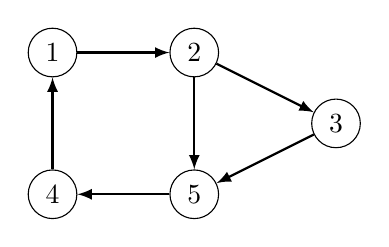
\begin{tikzpicture}[scale=0.9]
\node[draw, circle] (1) at (1,5) {$1$};
\node[draw, circle] (2) at (3,5) {$2$};
\node[draw, circle] (3) at (5,4) {$3$};
\node[draw, circle] (4) at (1,3) {$4$};
\node[draw, circle] (5) at (3,3) {$5$};

\path[draw,thick,->,>=latex] (1) -- (2);
\path[draw,thick,->,>=latex] (2) -- (3);
\path[draw,thick,->,>=latex] (4) -- (1);
\path[draw,thick,->,>=latex] (3) -- (5);
\path[draw,thick,->,>=latex] (2) -- (5);
\path[draw,thick,->,>=latex] (5) -- (4);
\end{tikzpicture}
\end{center}
los nodos 1, 3 y 4 tienen tanto grado de entrada 1 como grado de salida 1,
el nodo 2 tiene grado de entrada 1 y grado de salida 2,
y el nodo 5 tiene grado de entrada 2 y grado de salida 1.
Por lo tanto, el gráfico contiene un camino euleriano
desde el nodo 2 hasta el nodo 5:
\begin{center}
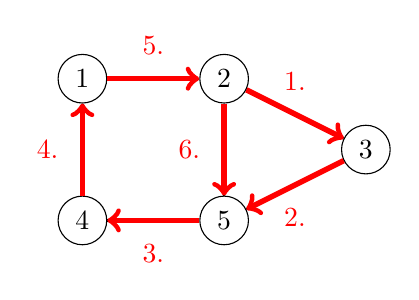
\begin{tikzpicture}[scale=0.9]
\node[draw, circle] (1) at (1,5) {$1$};
\node[draw, circle] (2) at (3,5) {$2$};
\node[draw, circle] (3) at (5,4) {$3$};
\node[draw, circle] (4) at (1,3) {$4$};
\node[draw, circle] (5) at (3,3) {$5$};

\path[draw,thick,-] (1) -- (2);
\path[draw,thick,-] (2) -- (3);
\path[draw,thick,-] (1) -- (4);
\path[draw,thick,-] (3) -- (5);
\path[draw,thick,-] (2) -- (5);
\path[draw,thick,-] (4) -- (5);

\path[draw=red,thick,->,line width=2pt] (2) -- node[font=\small,label={[red]north:1.}] {} (3);
\path[draw=red,thick,->,line width=2pt] (3) -- node[font=\small,label={[red]south:2.}] {} (5);
\path[draw=red,thick,->,line width=2pt] (5) -- node[font=\small,label={[red]south:3.}] {} (4);
\path[draw=red,thick,->,line width=2pt] (4) -- node[font=\small,label={[red]left:4.}] {} (1);
\path[draw=red,thick,->,line width=2pt] (1) -- node[font=\small,label={[red]north:5.}] {} (2);
\path[draw=red,thick,->,line width=2pt] (2) -- node[font=\small,label={[red]left:6.}] {} (5);
\end{tikzpicture}
\end{center}

\subsubsection{Algoritmo de Hierholzer}

\index{Algoritmo de Hierholzer}

\key{Algoritmo de Hierholzer}\footnote{El algoritmo fue publicado
en 1873 después de la muerte de Hierholzer \cite{hie73}.} es un método eficiente
para construir
un circuito euleriano.
El algoritmo consiste en varias rondas,
cada una de las cuales agrega nuevos bordes al circuito.
Por supuesto, asumimos que el gráfico contiene
un circuito euleriano; de lo contrario, el algoritmo de Hierholzer
no puede encontrarlo.

Primero, el algoritmo construye un circuito que contiene
algunos (no necesariamente todos) de los bordes del gráfico.
Después de esto, el algoritmo extiende el circuito
paso a paso agregando subcircuitos a él.
El proceso continúa hasta que se han agregado todos los bordes
al circuito.

El algoritmo extiende el circuito siempre buscando
un nodo $x$ que pertenece al circuito pero tiene
un borde saliente que no está incluido en el circuito.
El algoritmo construye un nuevo camino desde el nodo $x$
que solo contiene bordes que aún no están en el circuito.
Tarde o temprano,
el camino volverá al nodo $x$,
lo que crea un subcircuito.

Si el gráfico solo contiene un camino euleriano,
aún podemos usar el algoritmo de Hierholzer
para encontrarlo agregando un borde extra al gráfico
y eliminando el borde después de que el circuito
se haya construido.
Por ejemplo, en un gráfico no dirigido,
agregamos el borde extra entre los dos
nodos de grado impar.

A continuación, veremos cómo el algoritmo de Hierholzer
construye un circuito euleriano para un gráfico no dirigido.

\subsubsection{Ejemplo}
\begin{samepage}
Consideremos el siguiente gráfico:
\begin{center}
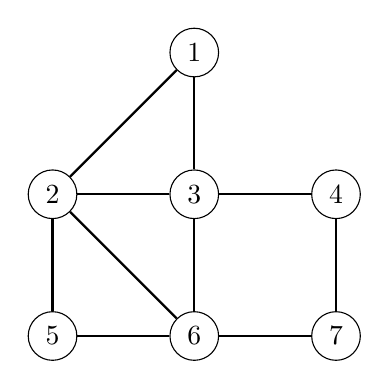
\begin{tikzpicture}[scale=0.9]
\node[draw, circle] (1) at (3,5) {$1$};
\node[draw, circle] (2) at (1,3) {$2$};
\node[draw, circle] (3) at (3,3) {$3$};
\node[draw, circle] (4) at (5,3) {$4$};
\node[draw, circle] (5) at (1,1) {$5$};
\node[draw, circle] (6) at (3,1) {$6$};
\node[draw, circle] (7) at (5,1) {$7$};

\path[draw,thick,-] (1) -- (2);
\path[draw,thick,-] (1) -- (3);
\path[draw,thick,-] (2) -- (3);
\path[draw,thick,-] (2) -- (5);
\path[draw,thick,-] (2) -- (6);
\path[draw,thick,-] (3) -- (4);
\path[draw,thick,-] (3) -- (6);
\path[draw,thick,-] (4) -- (7);
\path[draw,thick,-] (5) -- (6);
\path[draw,thick,-] (6) -- (7);
\end{tikzpicture}
\end{center}
\end{samepage}

\begin{samepage}
Supongamos que el algoritmo primero crea un circuito
que comienza en el nodo 1.
Un posible circuito es
$1 \rightarrow 2 \rightarrow 3 \rightarrow 1$:
\begin{center}
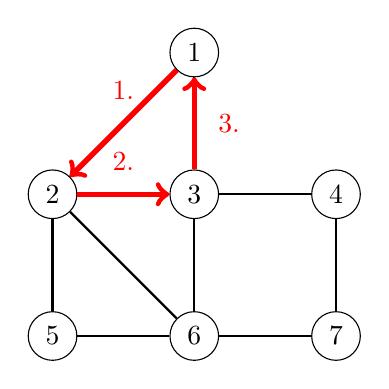
\begin{tikzpicture}[scale=0.9]
\node[draw, circle] (1) at (3,5) {$1$};
\node[draw, circle] (2) at (1,3) {$2$};
\node[draw, circle] (3) at (3,3) {$3$};
\node[draw, circle] (4) at (5,3) {$4$};
\node[draw, circle] (5) at (1,1) {$5$};
\node[draw, circle] (6) at (3,1) {$6$};
\node[draw, circle] (7) at (5,1) {$7$};

\path[draw,thick,-] (1) -- (2);
\path[draw,thick,-] (1) -- (3);
\path[draw,thick,-] (2) -- (3);
\path[draw,thick,-] (2) -- (5);
\path[draw,thick,-] (2) -- (6);
\path[draw,thick,-] (3) -- (4);
\path[draw,thick,-] (3) -- (6);
\path[draw,thick,-] (4) -- (7);
\path[draw,thick,-] (5) -- (6);
\path[draw,thick,-] (6) -- (7);

\path[draw=red,thick,->,line width=2pt] (1) -- node[font=\small,label={[red]north:1.}] {} (2);
\path[draw=red,thick,->,line width=2pt] (2) -- node[font=\small,label={[red]north:2.}] {} (3);
\path[draw=red,thick,->,line width=2pt] (3) -- node[font=\small,label={[red]east:3.}] {} (1);
\end{tikzpicture}
\end{center}
\end{samepage}
Después de esto, el algoritmo agrega
el subcircuito
$2 \rightarrow 5 \rightarrow 6 \rightarrow 2$
al circuito:
\begin{center}
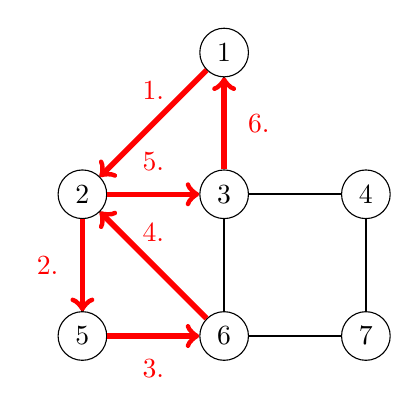
\begin{tikzpicture}[scale=0.9]
\node[draw, circle] (1) at (3,5) {$1$};
\node[draw, circle] (2) at (1,3) {$2$};
\node[draw, circle] (3) at (3,3) {$3$};
\node[draw, circle] (4) at (5,3) {$4$};
\node[draw, circle] (5) at (1,1) {$5$};
\node[draw, circle] (6) at (3,1) {$6$};
\node[draw, circle] (7) at (5,1) {$7$};

\path[draw,thick,-] (1) -- (2);
\path[draw,thick,-] (1) -- (3);
\path[draw,thick,-] (2) -- (3);
\path[draw,thick,-] (2) -- (5);
\path[draw,thick,-] (2) -- (6);
\path[draw,thick,-] (3) -- (4);
\path[draw,thick,-] (3) -- (6);
\path[draw,thick,-] (4) -- (7);
\path[draw,thick,-] (5) -- (6);
\path[draw,thick,-] (6) -- (7);

\path[draw=red,thick,->,line width=2pt] (1) -- node[font=\small,label={[red]north:1.}] {} (2);
\path[draw=red,thick,->,line width=2pt] (2) -- node[font=\small,label={[red]west:2.}] {} (5);
\path[draw=red,thick,->,line width=2pt] (5) -- node[font=\small,label={[red]south:3.}] {} (6);
\path[draw=red,thick,->,line width=2pt] (6) -- node[font=\small,label={[red]north:4.}] {} (2);
\path[draw=red,thick,->,line width=2pt] (2) -- node[font=\small,label={[red]north:5.}] {} (3);
\path[draw=red,thick,->,line width=2pt] (3) -- node[font=\small,label={[red]east:6.}] {} (1);
\end{tikzpicture}
\end{center}
Finalmente, el algoritmo agrega el subcircuito
$6 \rightarrow 3 \rightarrow 4 \rightarrow 7 \rightarrow 6$
al circuito:
\begin{center}
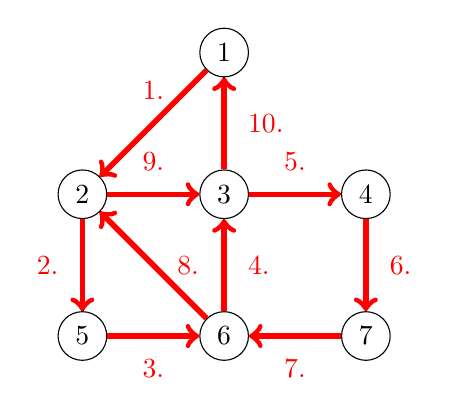
\begin{tikzpicture}[scale=0.9]
\node[draw, circle] (1) at (3,5) {$1$};
\node[draw, circle] (2) at (1,3) {$2$};
\node[draw, circle] (3) at (3,3) {$3$};
\node[draw, circle] (4) at (5,3) {$4$};
\node[draw, circle] (5) at (1,1) {$5$};
\node[draw, circle] (6) at (3,1) {$6$};
\node[draw, circle] (7) at (5,1) {$7$};

\path[draw,thick,-] (1) -- (2);
\path[draw,thick,-] (1) -- (3);
\path[draw,thick,-] (2) -- (3);
\path[draw,thick,-] (2) -- (5);
\path[draw,thick,-] (2) -- (6);
\path[draw,thick,-] (3) -- (4);
\path[draw,thick,-] (3) -- (6);
\path[draw,thick,-] (4) -- (7);
\path[draw,thick,-] (5) -- (6);
\path[draw,thick,-] (6) -- (7);

\path[draw=red,thick,->,line width=2pt] (1) -- node[font=\small,label={[red]north:1.}] {} (2);
\path[draw=red,thick,->,line width=2pt] (2) -- node[font=\small,label={[red]west:2.}] {} (5);
\path[draw=red,thick,->,line width=2pt] (5) -- node[font=\small,label={[red]south:3.}] {} (6);
\path[draw=red,thick,->,line width=2pt] (6) -- node[font=\small,label={[red]east:4.}] {} (3);
\path[draw=red,thick,->,line width=2pt] (3) -- node[font=\small,label={[red]north:5.}] {} (4);
\path[draw=red,thick,->,line width=2pt] (4) -- node[font=\small,label={[red]east:6.}] {} (7);
\path[draw=red,thick,->,line width=2pt] (7) -- node[font=\small,label={[red]south:7.}] {} (6);
\path[draw=red,thick,->,line width=2pt] (6) -- node[font=\small,label={[red]right:8.}] {} (2);
\path[draw=red,thick,->,line width=2pt] (2) -- node[font=\small,label={[red]north:9.}] {} (3);
\path[draw=red,thick,->,line width=2pt] (3) -- node[font=\small,label={[red]east:10.}] {} (1);
\end{tikzpicture}
\end{center}
Ahora todos los bordes están incluidos en el circuito,
por lo que hemos construido con éxito un circuito euleriano.

\section{Caminos hamiltonianos}

\index{camino hamiltoniano}

Un \key{camino hamiltoniano}
%\footnote{W. R. Hamilton (1805--1865) fue un matemático irlandés.}
es un camino
que visita cada nodo del grafo exactamente una vez.
Por ejemplo, el grafo
\begin{center}
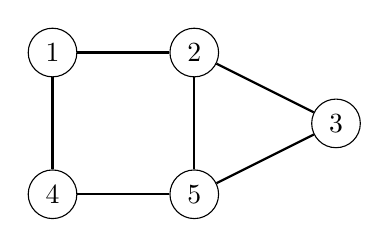
\begin{tikzpicture}[scale=0.9]
\node[draw, circle] (1) at (1,5) {$1$};
\node[draw, circle] (2) at (3,5) {$2$};
\node[draw, circle] (3) at (5,4) {$3$};
\node[draw, circle] (4) at (1,3) {$4$};
\node[draw, circle] (5) at (3,3) {$5$};

\path[draw,thick,-] (1) -- (2);
\path[draw,thick,-] (2) -- (3);
\path[draw,thick,-] (1) -- (4);
\path[draw,thick,-] (3) -- (5);
\path[draw,thick,-] (2) -- (5);
\path[draw,thick,-] (4) -- (5);
\end{tikzpicture}
\end{center}
contiene un camino hamiltoniano desde el nodo 1 hasta el nodo 3:
\begin{center}
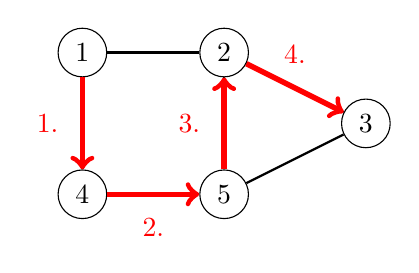
\begin{tikzpicture}[scale=0.9]
\node[draw, circle] (1) at (1,5) {$1$};
\node[draw, circle] (2) at (3,5) {$2$};
\node[draw, circle] (3) at (5,4) {$3$};
\node[draw, circle] (4) at (1,3) {$4$};
\node[draw, circle] (5) at (3,3) {$5$};

\path[draw,thick,-] (1) -- (2);
\path[draw,thick,-] (2) -- (3);
\path[draw,thick,-] (1) -- (4);
\path[draw,thick,-] (3) -- (5);
\path[draw,thick,-] (2) -- (5);
\path[draw,thick,-] (4) -- (5);

\path[draw=red,thick,->,line width=2pt] (1) -- node[font=\small,label={[red]left:1.}] {} (4);
\path[draw=red,thick,->,line width=2pt] (4) -- node[font=\small,label={[red]south:2.}] {} (5);
\path[draw=red,thick,->,line width=2pt] (5) -- node[font=\small,label={[red]left:3.}] {} (2);
\path[draw=red,thick,->,line width=2pt] (2) -- node[font=\small,label={[red]north:4.}] {} (3);
\end{tikzpicture}
\end{center}

\index{circuito hamiltoniano}

Si un camino hamiltoniano comienza y termina en el mismo nodo,
se llama \key{circuito hamiltoniano}.
El gráfico anterior también tiene un circuito hamiltoniano
que comienza y termina en el nodo 1:
\begin{center}
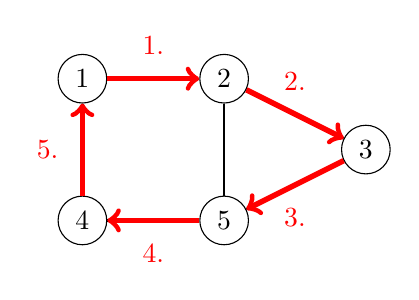
\begin{tikzpicture}[scale=0.9]
\node[draw, circle] (1) at (1,5) {$1$};
\node[draw, circle] (2) at (3,5) {$2$};
\node[draw, circle] (3) at (5,4) {$3$};
\node[draw, circle] (4) at (1,3) {$4$};
\node[draw, circle] (5) at (3,3) {$5$};

\path[draw,thick,-] (1) -- (2);
\path[draw,thick,-] (2) -- (3);
\path[draw,thick,-] (1) -- (4);
\path[draw,thick,-] (3) -- (5);
\path[draw,thick,-] (2) -- (5);
\path[draw,thick,-] (4) -- (5);

\path[draw=red,thick,->,line width=2pt] (1) -- node[font=\small,label={[red]north:1.}] {} (2);
\path[draw=red,thick,->,line width=2pt] (2) -- node[font=\small,label={[red]north:2.}] {} (3);
\path[draw=red,thick,->,line width=2pt] (3) -- node[font=\small,label={[red]south:3.}] {} (5);
\path[draw=red,thick,->,line width=2pt] (5) -- node[font=\small,label={[red]south:4.}] {} (4);
\path[draw=red,thick,->,line width=2pt] (4) -- node[font=\small,label={[red]left:5.}] {} (1);
\end{tikzpicture}
\end{center}

\subsubsection{Existencia}

No se conoce ningún método eficiente para probar si un gráfico
contiene un camino hamiltoniano, y el problema es NP-difícil.
Aún así, en algunos casos especiales, podemos estar seguros
de que un gráfico contiene un camino hamiltoniano.

Una simple observación es que si el gráfico es completo,
es decir, existe una arista entre todos los pares de nodos,
también contiene un camino hamiltoniano.
También se han logrado resultados más fuertes:

\begin{itemize}
\item
\index{Teorema de Dirac}
\key{Teorema de Dirac}: %\cite{dir52}
Si el grado de cada nodo es al menos $n/2$,
el gráfico contiene un camino hamiltoniano.
\item
\index{Teorema de Ore}
\key{Teorema de Ore}: %\cite{ore60}
Si la suma de grados de cada par de nodos no adyacentes
es al menos $n$,
el gráfico contiene un camino hamiltoniano.
\end{itemize}

Una propiedad común en estos teoremas y otros resultados es
que garantizan la existencia de un camino hamiltoniano
si el gráfico tiene \emph{un gran número} de aristas.
Esto tiene sentido, porque cuantas más aristas contiene el gráfico,
más posibilidades hay de construir un camino hamiltoniano.

\subsubsection{Construcción}
Dado que no existe una forma eficiente de comprobar si existe un 
camino hamiltoniano, es claro que tampoco existe un método 
para construir el camino de forma eficiente, porque de 
lo contrario, podríamos simplemente intentar construir el 
camino y ver si existe.

Una forma simple de buscar un camino hamiltoniano es utilizar un algoritmo 
de retroceso que recorre todas las formas posibles de construir el camino.
La complejidad temporal de dicho algoritmo es al menos $O(n!)$,
porque hay $n!$ formas diferentes de elegir el orden de $n$ nodos.

Una solución más eficiente se basa en la programación dinámica
(ver Capítulo 10.5).
La idea es calcular los valores
de una función $\texttt{posible}(S,x)$,
donde $S$ es un subconjunto de nodos y $x$
es uno de los nodos.
La función indica si existe un camino hamiltoniano
que visita los nodos de $S$ y termina en el nodo $x$.
Es posible implementar esta solución en $O(2^n n^2)$ tiempo.

\section{Secuencias de De Bruijn}

\index{Secuencia de De Bruijn}

Una \key{Secuencia de De Bruijn}
es una cadena que contiene
cada cadena de longitud $n$
exactamente una vez como subcadena, para un alfabeto fijo
de $k$ caracteres.
La longitud de dicha cadena es
$k^n+n-1$ caracteres.
Por ejemplo, cuando $n=3$ y $k=2$,
un ejemplo de una secuencia de De Bruijn es
\[0001011100.\]
Las subcadenas de esta cadena son todas
combinaciones de tres bits:
000, 001, 010, 011, 100, 101, 110 y 111.

Resulta que cada secuencia de De Bruijn
corresponde a un camino euleriano en un grafo.
La idea es construir un grafo donde
cada nodo contiene una cadena de $n-1$ caracteres
y cada arista agrega un carácter a la cadena.
El siguiente grafo corresponde al escenario anterior:

\begin{center}
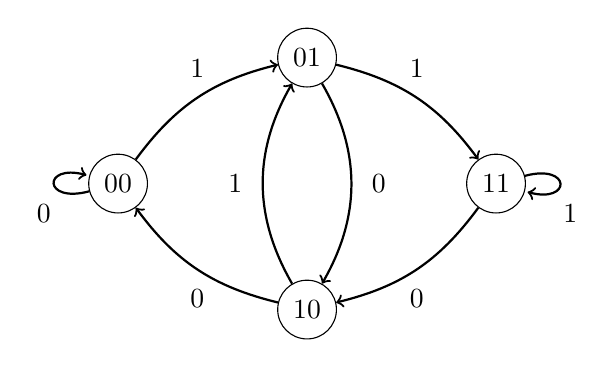
\begin{tikzpicture}[scale=0.8]
\node[draw, circle] (00) at (-3,0) {00};
\node[draw, circle] (11) at (3,0) {11};
\node[draw, circle] (01) at (0,2) {01};
\node[draw, circle] (10) at (0,-2) {10};

\path[draw,thick,->] (00) edge [bend left=20] node[font=\small,label=1] {} (01);
\path[draw,thick,->] (01) edge [bend left=20] node[font=\small,label=1] {} (11);
\path[draw,thick,->] (11) edge [bend left=20] node[font=\small,label=below:0] {} (10);
\path[draw,thick,->] (10) edge [bend left=20] node[font=\small,label=below:0] {} (00);

\path[draw,thick,->] (01) edge [bend left=30] node[font=\small,label=right:0] {} (10);
\path[draw,thick,->] (10) edge [bend left=30] node[font=\small,label=left:1] {} (01);

\path[draw,thick,-] (00) edge [loop left] node[font=\small,label=below:0] {} (00);
\path[draw,thick,-] (11) edge [loop right] node[font=\small,label=below:1] {} (11);
\end{tikzpicture}
\end{center}

Un camino euleriano en este grafo corresponde a una cadena
que contiene todas las cadenas de longitud $n$.
La cadena contiene los caracteres del nodo inicial
y todos los caracteres de las aristas.
El nodo inicial tiene $n-1$ caracteres
y hay $k^n$ caracteres en las aristas,
por lo que la longitud de la cadena es $k^n+n-1$.

\section{Recorridos del caballo}

\index{recorrido del caballo}

Un \key{recorrido del caballo} es una secuencia de movimientos
de un caballo en un tablero de ajedrez $n \times n$
siguiendo las reglas del ajedrez de modo que el caballo
visite cada casilla exactamente una vez.
Un recorrido del caballo se llama recorrido \emph{cerrado}
si el caballo finalmente regresa a la casilla inicial y
de lo contrario se llama recorrido \emph{abierto}.

Por ejemplo, aquí hay un recorrido abierto del caballo en un tablero de $5 \times 5$:

\begin{center}
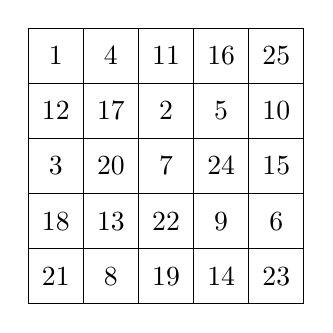
\begin{tikzpicture}[scale=0.7]
\draw (0,0) grid (5,5);
\node at (0.5,4.5) {$1$};
\node at (1.5,4.5) {$4$};
\node at (2.5,4.5) {$11$};
\node at (3.5,4.5) {$16$};
\node at (4.5,4.5) {$25$};
\node at (0.5,3.5) {$12$};
\node at (1.5,3.5) {$17$};
\node at (2.5,3.5) {$2$};
\node at (3.5,3.5) {$5$};
\node at (4.5,3.5) {$10$};
\node at (0.5,2.5) {$3$};
\node at (1.5,2.5) {$20$};
\node at (2.5,2.5) {$7$};
\node at (3.5,2.5) {$24$};
\node at (4.5,2.5) {$15$};
\node at (0.5,1.5) {$18$};
\node at (1.5,1.5) {$13$};
\node at (2.5,1.5) {$22$};
\node at (3.5,1.5) {$9$};
\node at (4.5,1.5) {$6$};
\node at (0.5,0.5) {$21$};
\node at (1.5,0.5) {$8$};
\node at (2.5,0.5) {$19$};
\node at (3.5,0.5) {$14$};
\node at (4.5,0.5) {$23$};
\end{tikzpicture}
\end{center}

Un recorrido del caballo corresponde a un camino hamiltoniano en un grafo
cuyos nodos representan las casillas del tablero,
y dos nodos están conectados con una arista si un caballo
puede moverse entre las casillas de acuerdo con las reglas del ajedrez.

Una forma natural de construir un recorrido del caballo es usar el retroceso.
La búsqueda se puede hacer más eficiente utilizando
\emph{heurísticas} que intentan guiar al caballo para que
se encuentre rápidamente un recorrido completo.

\subsubsection{Regla de Warnsdorf}

\index{heurística}
\index{Regla de Warnsdorf}
\key{Regla de Warnsdorf} es una heurística simple y efectiva
para encontrar un recorrido del caballo\footnote{Esta heurística fue propuesta
en el libro de Warnsdorf \cite{war23} en 1823. También hay
algoritmos polinomiales para encontrar recorridos del caballo
\cite{par97}, pero son más complicados.}.
Usando la regla, es posible construir eficientemente un recorrido
incluso en un tablero grande.
La idea es siempre mover el caballo de modo que termine
en un cuadrado donde el número de movimientos posibles es
\emph{lo más pequeño} posible.

Por ejemplo, en la siguiente situación, hay cinco
cuadrados posibles a los que el caballo puede moverse (cuadrados $a \ldots e$):
\begin{center}
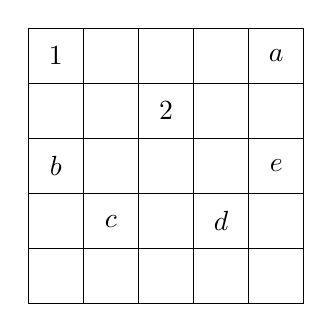
\begin{tikzpicture}[scale=0.7]
\draw (0,0) grid (5,5);
\node at (0.5,4.5) {$1$};
\node at (2.5,3.5) {$2$};
\node at (4.5,4.5) {$a$};
\node at (0.5,2.5) {$b$};
\node at (4.5,2.5) {$e$};
\node at (1.5,1.5) {$c$};
\node at (3.5,1.5) {$d$};
\end{tikzpicture}
\end{center}
En esta situación, la regla de Warnsdorf mueve el caballo al cuadrado $a$,
porque después de esta elección, solo hay un movimiento posible.
Las otras opciones moverían el caballo a cuadrados donde
habría tres movimientos disponibles.
